\chapter{Theoretischer Hintergrund}

\section{Lerntypeneinteilung nach Gagné}

Gagné unterteilt seine Formen des Lernens hierarchisch, somit setzt meist die nachfolgende Lernart die vorhergehenden Lernarten voraus. Generell wird in zwei Teile unterteilt: 
\begin{itemize}
\item (A) Grundformen der Lernens: Assoziationen und Ketten 
    \begin{itemize}
        \item (A.1) Signallernen
        \item (A.2) Reiz-Reaktions-Lernen
        \item (A.3) Kettenbildung
        \item (A.4) Sprachliche Assoziation
    \end{itemize}
\item (B) Intellektuelle Fähigkeiten
    \begin{itemize}
        \item (B.1) Diskriminationslernen
        \item (B.2) Begriffslernen
        \item (B.3) Regellernen 
        \item (B.4) Problemlösen
    \end{itemize}
\end{itemize}

\subsection[]{(A.1) Signallernen (Pawlos "klassische" Konditionierungslehre)}

Man versucht mit einem Reiz eine dadurch bedingte Reaktion hervorzurufen. Eines der bekanntesten pädagogischen Phänomene hierfür ist der "Pawlowsche Hund". Hierbei wird immer bevor ein Hund Futter bekommt eine Glocke geschlagen. Nach vielen Druchgängen wird nur noch die Glocke geschlagen, was eine den Speichelfluss des Hundes anreizt, ohne das er Futter bekommt. Somit können einfache Reize ( z.B Ton) bestimmte Reaktionen (z.B Speichelfluss), welche nicht reflexartig angeboren sind, sondern an trainiert wurden, hervorrufen. %\cite Pawlos Konditionierungslehre

\subsection[]{(A.2) Reiz-Reaktions-Lernen (Trial and Error Prinzip, Lernen durch Verstärkung)}

Der Lernende versucht etwas so lang auf verschiedene Art und Weißen, bis es klappt und merkt sich anschließend wie man es gemacht hat. 
Beispiel: Jemand ist sich bei der letzten Nummer seines Fahrradschlosses unsicher. Er versucht deswegen einfach alle Möglichkeiten von 0 - 9 und merkt sich bei welcher Zahl das Schloss aufgegangen ist. Hierbei erfährt der Lernende eine Verstärkung, weil er danach mehr kann als davor ( in unserem Beispiel :Schloss öffnen) und dies nur durch einfaches Ausprobieren geschafft hat.

\subsection[]{(A.3) Kettenbildung (Lernen von Abläufen)}

In diesem Fall werden längere Reiz-Reaktions-Ketten gebildet. Hierbei sind alle Formen von Algorithmen oder Verfahren gemeint. Beispiele: Kochen, Telefonieren, oder auch Klammern im Mathematikunterricht auflösen. Diese Ketten können meist verstanden und durchgeführt werden, ohne einen tieferen Sinn des einzelnen Verfahrens verstanden zu haben. In der Schule kann diese Lernart zu Problemen führen, da die SuS (Schüler und Schülerinnen) kein Verständnis für die Zusammenhänge haben müssen, sondern nur ihre Algorithmen durchgehen können. Dies kann in Aufgaben mit höherem Abstraktionsgrad zu Problemen führen, wenn ihr Schema nicht mehr ohne weiteres anwendbar ist.

\subsection[]{(A.4) Sprachliche Assoziation (verbales auswendig Lernen)}

Hierbei werden bestimmte Definitionen, Gedichte oder Ähnliches einfach so lange wiederholt, bis sie auswendig vom Lernenden vorgetragen werden können. Hierbei findet somit eine Verkettung oder auch Assoziation von einfachen Objekten, in unserem Fall Wörtern, statt. Hierbei ist werden ebenso, wie in den anderen Grundformen, lediglich die Verknüpfungen der Wörter geschaffen und kein Verständnis dabei erzeugt. 

\subsection[]{(B.1) Diskriminationslernen (Unterscheidungslernen)}

In diesem Fall soll der Lernende verschiedene Gegenstände und Merkmale als verschieden auffassen können. Beispiele: Ein bestimmtes Passwort passt nur zu einem bestimmten Account, oder: nicht jedes Fahrrad schaut gleich aus, es gibt Rennräder, Stadträder, Lastenräder uvm.  . Somit soll der Lernende in besseres Verständnis für Begriffe entwickeln, indem er lernt diese zu differenzieren.

\begin{figure}[!ht]
\noindent\hspace{0.5mm}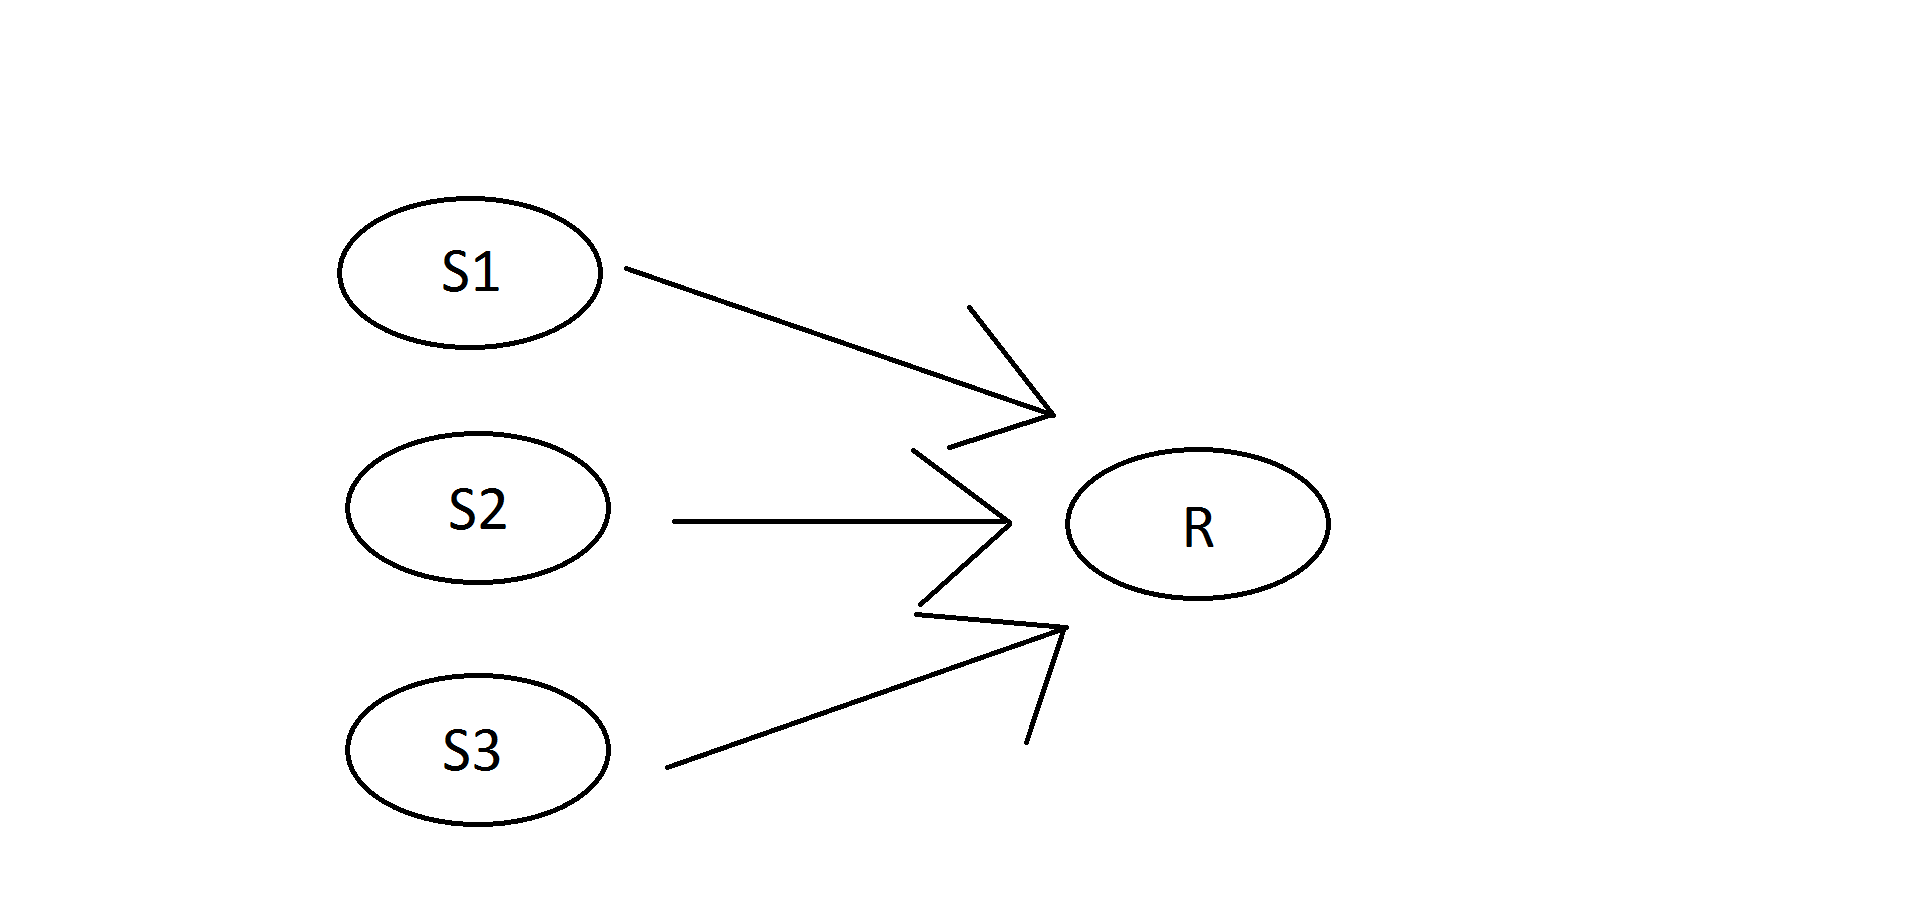
\includegraphics[width=12cm]{./Ressourcen/Diskrimination.png}
\caption{Diskriminationsleren, Zech}
\end{figure}

\subsection[]{(B.2) Begriffslernen (Gemeinsamkeiten finden)}

Bei diesem Typ soll genau der andere Weg wie im Diskriminationslernen gegangen werden. Hierbei sollen unterschiedliche Objekte als gleich zusammengefasst werden können. 
Beispiele: ein Rechteck und ein Quadrat sind beides Vierecke, oder ein Audi Q7 und ein BMW 5er sind beides Autos. Somit können besser Verbindungen zwischen Lerngegenständen hergestellt werden und sich auf allgemeine Details zurückgezogen werden (z.B Winkelsumme Viereck sind 360 Grad, Auto hat einen Motor).

\begin{figure}[!ht]
\noindent\hspace{0.5mm}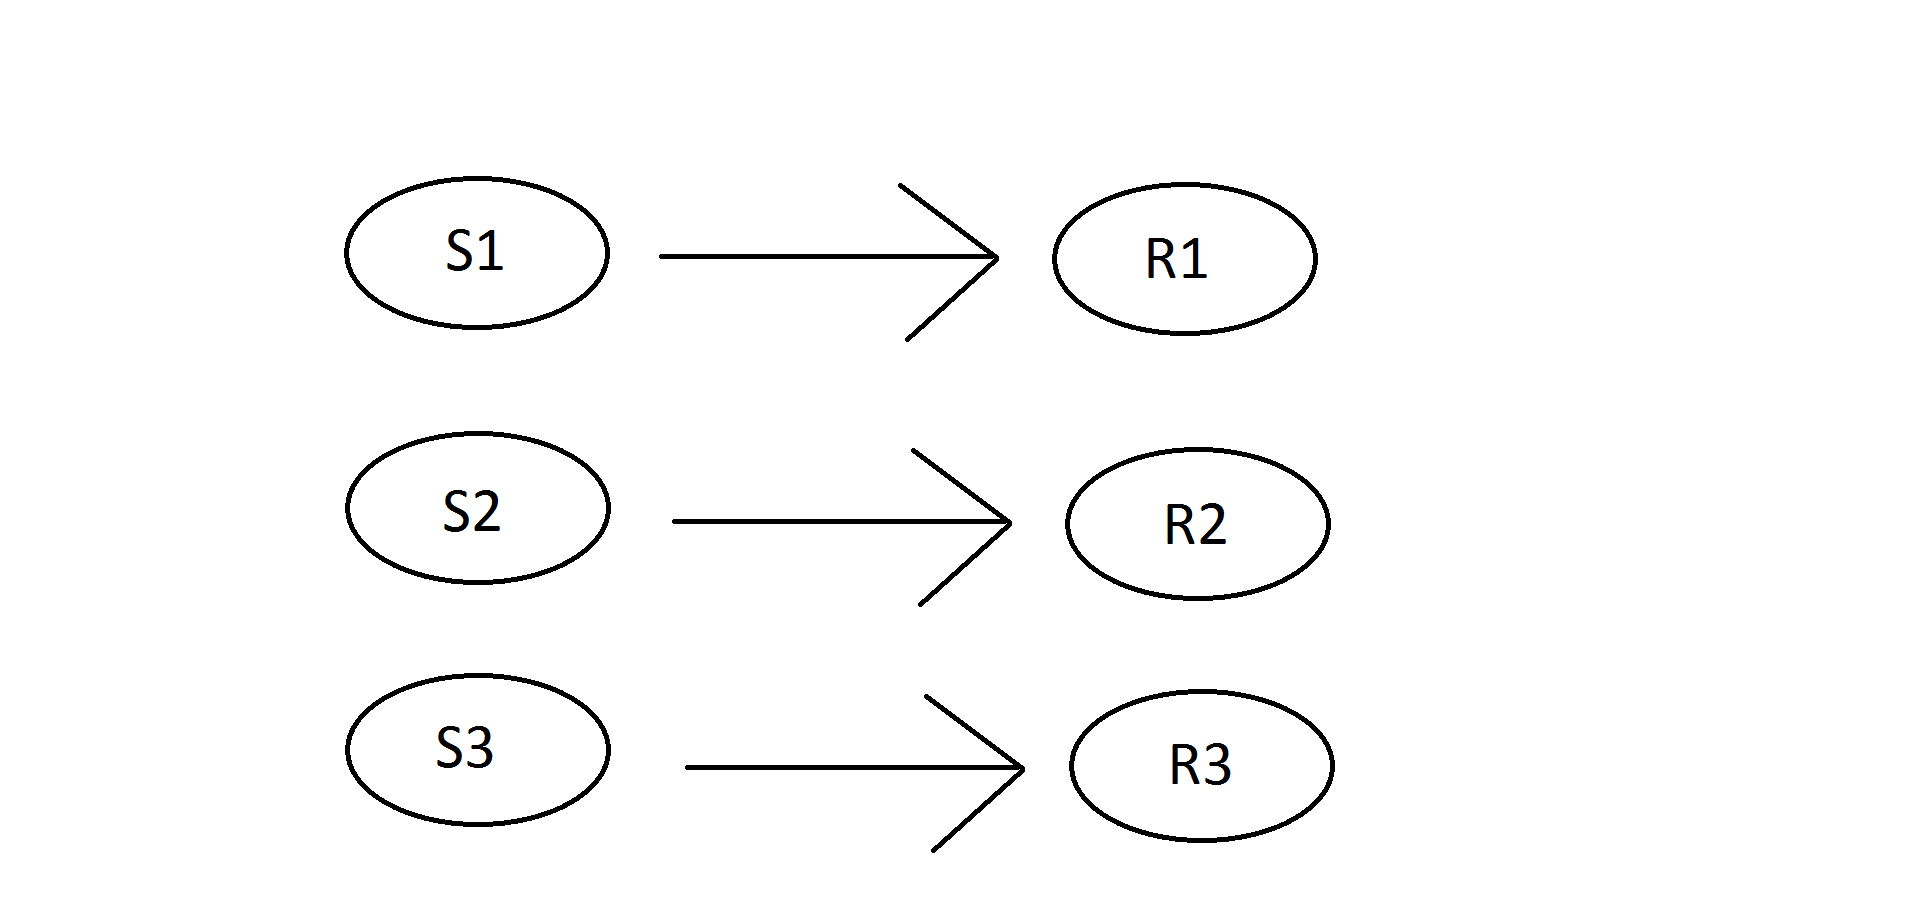
\includegraphics[width=12cm]{./Ressourcen/Begriffslernen.png}
\caption{Begriffslernen, Zech}
\end{figure}

\subsection[]{(B.3) Regellernen (Regeln auf Anwendungsbereiche lernen)}

Hierbei ist nicht nur das einfache auswendig lernen von Regeln oder der gleichen gemeint, sondern auch das damit verbundene Verständnis. Somit kann das Regellernen als im Kontext des Satzes von Pythagoras aufgefasst werden: Das zum einen die Formel $a^2$ + $b^2$ = $c^2$ im aktiven Wissen vorhanden ist, als auch die Anwendung und die Bedingungen der Formel verständlich sind.

\subsection[]{(B.4) Problemlösen (Aufgaben mit eigenen Überlegungen lösen)}

Dies ist der nächste Schritt von dem Regellernen, da hierbei Regeln verstanden sein müssen und diese kombiniert in einer Aufgabe angewendet werden können. Somit gehört in der gagnéschen Hierarchie der Problemlöser zur höchsten Ordnung, da seine Kompetenzen die Kompetenzen der vorhergehenden Typen beinhalten.

\section{Lerntypeneinteilung nach Zech}

Die Lerntypen von Gagné werden in der Einteilung nach Zech aufgegriffen, zusammengefasst und erweitert um neue Lerntypen zu definieren. Ebenso betrachtet er die Lerntypen hauptsächlich im Kontext der Mathematik und nicht mehr Allgemeinen. Zech unterteilt seine Lerntypen nicht mehr Hierarchisch wie zuvor passiert ist und gibt klare Lernbedienungen für den jeweiligen Lerntypen an. Es werden die folgenden 7 Typen betrachtet:

\subsection[]{Assoziatives Lernen}

In dieser Unterteilung sind die im kognitiven Bereich beschränkten Grundformen des Lernens (Teil A) nach Gagné zusammengefasst. Somit werden bei diesem Typ "kürzere oder längere Reiz-Reaktions-Verbindungen (Automatismen)" aufgebaut und diese hauptsächlich auswendig gelernt. Dies kann man im Mathematischen Sinne als das Anwenden von bekannten Regeln auf einfache Aufgabentypen verstanden werden. Ebenso bezieht sich dieser Typ über die Abstammung von den Grundformen (A) mehr auf textuelle Teile von Aufgaben, als auf bildliche Teile.
Die Lernbedingung dieses Types ist: häufige Wiederholung. 
Aus diesem Typ entsteht in der Unterteilung des Versuchaufbaus dieser Arbeit die Gruppierung "Textueller", welche sich dadurch auszeichnet das heuristische Beispiel sehr häufig wiederholt durchliest und sich somit, nach dem ersten durchlesen weiter auf den Text fokussiert. 


\subsection[]{Diskriminationslernen}

Er wird zu großen Teilen aus dem Typ von B.1 abgeleitet, wie der Name auch schon vermuten lässt. Hierbei wird aber nochmal verdeutlicht, dass das Diskriminationslernen als Voraussetzung zum Begriffslernen stehen muss, da erst Objekte unter einem Begriff zusammengefasst werden können, bevor sie als unterschiedlich erkannt werden können.
Lernbedingungen: Unterschiede hervorheben (zum Beispiel mit bunter Kreide), Kontiguität (Angrenzung, Berührung)%\cite"https://www.duden.de/rechtschreibung/Kontiguitaet".
Dieser Lerntyp ist in der gegebenen Studie schwer von den anderen Typen zu unterscheiden, da sich die Aufgabenstellung nicht explizit mit Diskrimination befasst, sondern mit dem lösen mathematischer Probleme. Somit wird dieser Lerntyp in der Studie nicht weiter behandelt.

\subsection[]{Lernen mathematischer Begriffe}

Dieser Typ baut sich auch auf dem Lerntyp B.2 Begriffslernen auf. Hierbei werden vorerst die Begriffe unterteilt in: Eigenschaftsbegriffe, Relationsbegriffe und zusammengesetzte Begriffe. Eigenschaftsbegriffe beschreiben Merkmale oder Eigenschaften eines Objektes. Relationsbegriffe beschreiben eine Relation zwischen verschiedenen Objekten, wie z.B A hat mehr Kanten wie B. Zusammengesetzte Begriffe werden aus einer Kombination von ursprünglichen Begriffen definiert z.B \textit{ eine Teilmenge des euklidischen Raums R n heißt kompakt, wenn sie abgeschlossen und beschränkt ist}. Diese Begriffe sollen durch die zusammenstezung mehrere bekannter Begriffe verstanden werden. Dieser Lerntyp auf B.3 Regellernen auf. Die Begriffe gehen durch Abstraktion aus der Erfahrungswelt hervor.
Lernbedingungen: relevante Merkmale hervorheben, mehrere Beispiele(irrelevante Merkmale variieren), Gegenbeispiele.
Leider sind die gegebenen Lernbedingungen an Hand einer Eyetracking-Studie, bei der nichts markiert werden kann, oder der Proband Beispiele und Gegenbeispiele anbringen kann, nicht auszuwerten. Aus diesem Grund wurde dieser Lerntyp ebenso in der Studie nicht weiter behandelt. 

\subsection[]{Lösen mathematischer Probleme}

Unter diesem Lerntyp wird ein verinnerlichen mathematischer Zusammenhänge verstanden. Hierbei wird das lernen von heuristischer Regeln vorausgesetzt. Es müssen zuerst bestimmte allgemeine Strategien (z.B Widerspruchsbeweis) aufgenommen werden, um anschließend eine Transferleistung zu vollbringen, wie es in Aufgaben mit hohem Abstraktionsgrad vorausgesetzt wird. 
Lernbedingungen: Problemlösefahigkeiten (analysieren, vergleichen, Beziehungen herstellen uvm), Fähigkeit, heuristische Regeln einzusetzen.
In Anlehnung an den Typ "Lösen mathematischer Probleme" wird in meiner Arbeit die Gruppierung "Problemlöser" definiert, welche sich sehr stark auf die Bilder fokussiert nachdem er den Text das erste mal durchgelesen hat.

\section{Lerntypeneinteilung nach Schrader}

Wie bereits angedeutet unterteilt Schrader seine Lerntypen eher in Sozialformen: der Theoretiker, der Anwendungsorientierte, der Musterschüler, der Gleichgültige und der Unsichere. Hierbei werden nicht mehr alle Typen aufgelistet, da viele sich in den Typen von Zech widerspiegeln und in der Studie nicht die Sozialformen berücksichtigt wurden. Somit wird nur auf den Typ "der Unsichere" eingegangen.

Der "Unsichere" sucht Ursachen bei sich und zweifelt an seinen Fähigkeiten. Das lernen aus Texten fällt diesem Typ schwer, da er wenig systematisch dabei vorgeht. Er lässt sich lieber etwas mehr Zeit und die gegebene Aufgabenstellung zu bearbeiten.
Lerncharakteristik: Da ihm das arbeiten mit Texten Schwierigkeiten bereitet, ist die Bearbeitungszeit länger als gewöhnlich und es werden sowohl im textuelle Bereiche als auch Bildbereiche häufiger betrachtet, als bei einem gewöhnlichen Probanden es der Fall wäre. 

\section{Mehrgewinn von Graphischen Darstellungen}

Laut einer Studie von (Mayer,2005), hat das Arbeitsgedächtniss zwei Kanäle zur Verarbeitung von Informationen. Einer der Kanäle verarbeitet Informationen von Wörtern und der andere von Bildern. Somit kann eine optimale Lernbedingung geschafft werden, indem sowohl verständlicher Text als auch passende (eingebundene) Bilder dem Lernenden zu Verfügung gestellt werden. Laut Matthias Böckmann und Stanislaw Schukajlow (2018) lassen sich Bilder in drei unterschiedliche Typen unterteilen:
    
    \begin{itemize}
        \item dekorative Bilder (Decorative pictures), welche keine echten Informationen über das gegeben Problem geben. Zum Beispiel eine Radfahrerin, wenn es in der Aufgabe über das Zurücklegen einer Strecke mit dem Rad geht.
        \item repräsentative Bilder (Representational pictures), welche Teile der gestellten Aufgabe veranschaulichen. Zum Beispiel ein Drachenviereck, wenn die Aufgabe gestellt ist: den Flächeninhalt eines Drachenvierecks zu bestimmen. 
        \item essenzielle Bilder (Essential pictures), welche Informationen geben die essenziell sind für die Bearbeitung der Aufgabe. Zum Beispiel bei der Berechnung einer Fläche, ein Graphik in der relevante längen von Seiten eingetragen sind.
    \end{itemize}

In ihrer Studie wurden 217 SuS aus der 9. Klasse in Gruppen eingeteilt. Bei dem Versuch wurden die SuS in drei Gruppen unterteilt, welche die selbe Aufgabenstellung bekommen haben, jedoch die Bildtypen sich unterschieden haben. In der Aufgabe wird von den SuS verlangt den Abstand von einer Person zu ihrem Lenkdrachen, mit hilfe des Satzes von Pythagoras, zu berechnen. Die Aufgabestellung sollte von den SuS nicht bearbeitet, sondern lediglich Fragen hierzu beantwortet werden. 
Die erste Gruppe hat eine Aufgabenstellung mit einem dekorativen Bild gestellt bekommen. Hierbei ist nur ein Bild eines Lenkdrachen gezeigt.
Die zweite Gruppe hat ein Bild erhalten in dem die beschriebene Situation bildlich dargestellt wurde (repräsentativ). Hingegen hat die dritte Gruppe das selbe Bild wie die zweite Gruppe erhalten, nur mit längenangaben im Bild (essenziell).
Es konnte gezeigt werden, dass dekorative Bilder den Probanden kaum eine Unterstützung in der Lösung der gestellten Aufgaben geben. Hingegen repräsentative einen positiven Effekt haben und essenzielle Bilder den besten Effekt haben.%cite
